\documentclass[11pt]{article}

\usepackage[utf8]{inputenc}
\usepackage[T1]{fontenc}
\usepackage{amsmath,amssymb}
\usepackage{graphicx}
\usepackage{booktabs}
\usepackage{natbib}
\usepackage[breaklinks=true]{hyperref}
\usepackage{url}
\Urlmuskip=0mu plus 1mu
\usepackage{xcolor}
\usepackage{geometry}
\usepackage{float}
\usepackage{multirow}
\usepackage{caption}
\usepackage{subcaption}
\usepackage{algorithm}
\usepackage{algpseudocode}
\usepackage{setspace}

\geometry{margin=1in, headheight=15pt}
\bibliographystyle{abbrvnat}
\setcitestyle{authoryear,open={(},close={)}}

% JAMES-style formatting (1.5 spacing)
\setstretch{1.5}
\raggedbottom

% Section spacing
\usepackage{titlesec}
\titlespacing*{\section}{0pt}{1.2\baselineskip}{0.8\baselineskip}
\titlespacing*{\subsection}{0pt}{1.0\baselineskip}{0.6\baselineskip}
\titlespacing*{\subsubsection}{0pt}{0.9\baselineskip}{0.5\baselineskip}

% Caption styling
\captionsetup{font=small,labelfont=bf,margin=10pt}
\captionsetup[sub]{font=small}

\title{A Pioneering AI Land Surface Model for Subseasonal-to-Seasonal Prediction}

\author{Manmeet Singh$^{1}$, Nachiketa Acharya$^{2}$, Priyanka Yadav$^{3,4}$, Josh Durkee$^{1}$, \\
Somnath Luitel$^{1}$, Sanjiv Kumar$^{5}$, Zong-Liang Yang$^{7}$, Cenlin He$^{6}$, \\
Naveen Sudharsan$^{7}$, Harsh Kamath$^{8}$, Mahmoud Mbarak$^{9}$, \\
Prabhjot Singh$^{7}$, Amit Srivastava$^{10}$ \\
\small $^{1}$Western Kentucky University; $^{2}$Spire Global, Inc.; $^{3}$UMD ESSIC; $^{4}$NASA GSFC; \\
\small $^{5}$Auburn University; $^{6}$NCAR; $^{7}$UT Austin; $^{8}$NOAA; $^{9}$Duke University; $^{10}$ZALF
}

\date{\today}

\begin{document}
\maketitle

\section*{Key Points}
\begin{enumerate}
    \item We introduce Earthmind-Land, the first standalone modular AI land surface model for coupled Earth system forecasting.
    \item The model produces skillful 60-day forecasts of soil moisture and temperature across high-impact extreme weather events.
    \item Successful offline validation establishes a modular component ready for integration into coupled AI weather and climate systems.
\end{enumerate}

% =====================================================================
\begin{abstract}
Land surface processes govern critical memory mechanisms---soil moisture, soil temperature, and snow---that underpin subseasonal-to-seasonal (S2S) predictability. However, the recent revolution in AI-based weather and climate models has focused almost exclusively on the atmosphere, leaving no modular AI land surface model available for coupling with other AI components. We present the first standalone AI land surface model designed as a modular component for coupled AI earth system modeling. The model is trained on ERA5 reanalysis data (native resolution 0.25$^\circ$), regridded to a global Hierarchical Equal Area isoLatitude Pixelisation (HEALPix) grid at 0.7$^\circ$ resolution for processing, taking 9 atmospheric forcing variables and 8 soil state variables at time $t$ and predicting the land surface state at time $t+1$ (one day ahead): soil moisture across 4 soil layers and soil temperature across 4 levels. Data are accessed via cloud-native infrastructure, requiring no local downloads. In offline prediction mode---where observed atmospheric forcing from ERA5 is provided at each time step while the model evolves its own land surface state---the model produces skillful 60-day forecasts of soil moisture and soil temperature, validated across four extreme events: the 2019 Mississippi River basin flooding, the 2012 Central US drought, the 2021 Pacific Northwest heat dome, and the 2011 Texas drought, spanning 16 initializations. The model maintains anomaly correlation coefficients above 0.5 beyond 30 days for surface soil moisture, demonstrating its viability as the land component of coupled AI S2S prediction systems and offering the potential to be integrated into any physics-based or AI-based coupled model.
\end{abstract}

\section*{Plain Language Summary}
Predicting weather and climate weeks in advance depends on ``memory'' stored in the soil, such as moisture and temperature. While AI has revolutionized atmospheric weather forecasting, it has largely ignored the land surface. We have developed the first modular AI-based land surface model, called Earthmind-Land. This model learns how soil moisture and temperature change over time by looking at historical data. We tested it on major events like the 2012 US drought and 2021 heatwaves. Our results show that the model can accurately predict soil conditions up to two months in advance. Because the model is modular, it can be plugged into other AI systems to create complete forecasts of the Earth's atmosphere, land, and oceans. This work fills a major gap in modern AI weather systems and provides a faster, efficient way to predict environmental extremes.

% =====================================================================
\section{Introduction}
\label{sec:intro}

The land surface exerts a profound influence on weather and climate across a wide range of timescales. Soil moisture, in particular, acts as a source of predictability at subseasonal-to-seasonal (S2S) scales through its control on the partitioning of surface energy and water fluxes \citep{koster2004glace, seneviratne2010landclimate, dirmeyer2011landatm}. The Global Land--Atmosphere Coupling Experiment (GLACE) demonstrated that realistic soil moisture initialization can improve precipitation forecast skill weeks into the future \citep{koster2004glace}. Soil temperature, though less studied in this context, similarly provides memory through its coupling with surface energy balance and freeze--thaw processes. These land surface memory mechanisms are central to S2S prediction \citep{vitart2017s2s, merryfield2020s2s}.

Over the past four decades, the geoscience community has developed sophisticated physics-based land surface models (LSMs) to represent these processes. Models such as Noah-MP \citep{niu2011noahmp, ek2003noah}, the Community Land Model (CLM5; \citealt{lawrence2019clm5}), and the Joint UK Land Environment Simulator (JULES; \citealt{best2011jules}) solve coupled energy and water balance equations across multiple soil layers, incorporating vegetation dynamics, snow physics, and increasingly, groundwater and biogeochemical cycles. These models are typically developed and validated in offline mode---driven by observed or reanalysis atmospheric forcing---before being coupled into general circulation models (GCMs) for weather and climate prediction \citep{bauer2015quietrev}.

Concurrently, the past five years have witnessed a revolution in AI-based weather prediction. Beginning with early demonstrations using convolutional neural networks \citep{weyn2019dlwp, weyn2020dlwpcs}, the field rapidly advanced through Pangu-Weather \citep{bi2023pangu}, GraphCast \citep{lam2023graphcast}, FourCastNet \citep{pathak2022fourcastnet}, Spherical Fourier Neural Operators \citep{bonev2023sfno}, FuXi \citep{chen2023fuxi}, and Aurora \citep{bodnar2024aurora}. These models have demonstrated forecast skill competitive with---and in many metrics exceeding---operational numerical weather prediction systems such as ECMWF's Integrated Forecasting System, as documented by the WeatherBench~2 benchmark \citep{rasp2024weatherbench2}. More recently, NeuralGCM has shown that AI-based atmospheric dynamics can be combined with physical parameterizations for stable long-term climate simulations \citep{kochkov2024neuralGCM}.

A critical observation, however, is that nearly all of these AI weather models operate exclusively on atmospheric variables. They do not contain separate, identifiable land surface components. While some models (e.g., NeuralGCM) include land surface embeddings within their architectures, these are not modular components that can be independently developed, validated, or coupled. The first coupled AI ocean--atmosphere model, OLA \citep{caillon2024ola}, demonstrated the viability of training separate AI models for ocean and atmosphere on a shared grid and coupling them at inference time---but did not include a land component. Similarly, efforts in AI-based S2S prediction, such as FuXi-S2S \citep{chen2024fuxis2s}, have begun incorporating land surface variables but without a standalone, separable land model component.

This gap motivates the present work. We introduce the first standalone AI land surface model designed as a modular component for coupled AI earth system modeling. No such AI-based land surface model existed prior to this work. The model is explicitly designed to be modular: it can be integrated into any coupled AI or physics-based forecasting system that operates on a compatible grid. Following the time-honored development philosophy of physics-based LSMs---offline validation before coupled integration---we present the model in offline mode, forced by ERA5 atmospheric reanalysis data. The model is built as part of the Earthmind S2S framework, which aims to couple independent AI models for atmosphere, land, and ocean on a common grid.

The key contributions of this work are:
\begin{enumerate}
    \item The first standalone AI land surface model, which did not exist in the literature prior to this work. The model fills a critical gap in coupled AI earth system modeling.
    \item A neural network architecture adapted for global land surface modeling on a global equal-area grid, treating the 12 grid faces as a depth dimension in 3D convolutions, enabling shared-grid coupling with AI atmosphere and ocean models.
    \item A cloud-native training pipeline that streams ERA5 reanalysis data directly from cloud-optimized storage, eliminating the need for local data infrastructure.
    \item Demonstration of skillful autoregressive offline forecasts of soil moisture and soil temperature out to 60 days across four high-impact extreme events (flooding, drought, heat) at S2S timescales.
    \item An open, modular design that enables the model to be plugged directly into any coupled forecasting system---whether physics-based or AI-based---with minimal adaptation, advancing the modularity paradigm in earth system modeling.
\end{enumerate}

% =====================================================================
\section{Data and Variables}
\label{sec:data}

The model is trained and evaluated using the ERA5 global reanalysis \citep{hersbach2020era5}, accessed through the ARCO-ERA5 dataset \citep{carver2023arcoera5}. The native ERA5 data are provided at 0.25$^\circ$ horizontal resolution. For training, we aggregate hourly data to daily means.

The model takes 17 input variables and predicts 8 target variables (Table~\ref{tab:variables}). The input variables consist of 9 atmospheric forcing fields and 8 soil state variables at time $t$. The target variables are the same 8 soil state variables at time $t+1$. The soil variables span four vertical layers in ERA5: Layer~1 (0--7~cm), Layer~2 (7--28~cm), Layer~3 (28--100~cm), and Layer~4 (100--289~cm).

\begin{table}[htbp]
\centering
\caption{Input and target variables used in the Earthmind-Land model.}
\label{tab:variables}
\small
\begin{tabular}{@{}llcrr@{}}
\toprule
\textbf{Variable} & \textbf{Role} & \textbf{Unit} & \textbf{Min} & \textbf{Max} \\
\midrule
2\,m temperature & Input & K & 188.0 & 326.9 \\
Total precipitation & Input & m & 0.0 & 0.101 \\
10\,m $u$-wind & Input & m\,s$^{-1}$ & $-$281.1 & 132.5 \\
10\,m $v$-wind & Input & m\,s$^{-1}$ & $-$159.2 & 166.6 \\
Surface solar radiation downwards & Input & J\,m$^{-2}$ & $-$6.0 & $4.89\times10^6$ \\
Evaporation & Input & m & $-$0.0028 & 0.0007 \\
Skin temperature & Input & K & 185.8 & 347.6 \\
Snowfall & Input & m & 0.0 & 0.016 \\
Mean sea level pressure & Input & Pa & 89991 & 109923 \\
\midrule
Vol.\ soil water layer 1--4 & I/O & m$^3$\,m$^{-3}$ & --- & --- \\
Soil temperature level 1--4 & I/O & K & --- & --- \\
\bottomrule
\end{tabular}
\end{table}

\subsection{Preprocessing}

Preprocessing includes temporal aggregation to daily means, MinMax normalization to the $[0, 1]$ range, and ocean filling using bilinear interpolation.

% =====================================================================
\section{Methods}
\label{sec:methods}

\subsection{HEALPix Grid Representation}

We represent global fields on the HEALPix grid at level 6 ($12 \times 64 \times 64 = 49{,}152$ pixels). HEALPix offers equal area and no polar singularity. Regridding is performed using the NVIDIA \texttt{earth2grid} library.

\subsection{3D UNet Architecture}

The core is a 3D UNet architecture with 4.5 million parameters. The 12 HEALPix faces are treated as a depth dimension for 3D convolutions. The model uses an encoder--decoder structure with skip connections (Figure~\ref{fig:architecture}).

\begin{figure}[htbp]
    \centering
    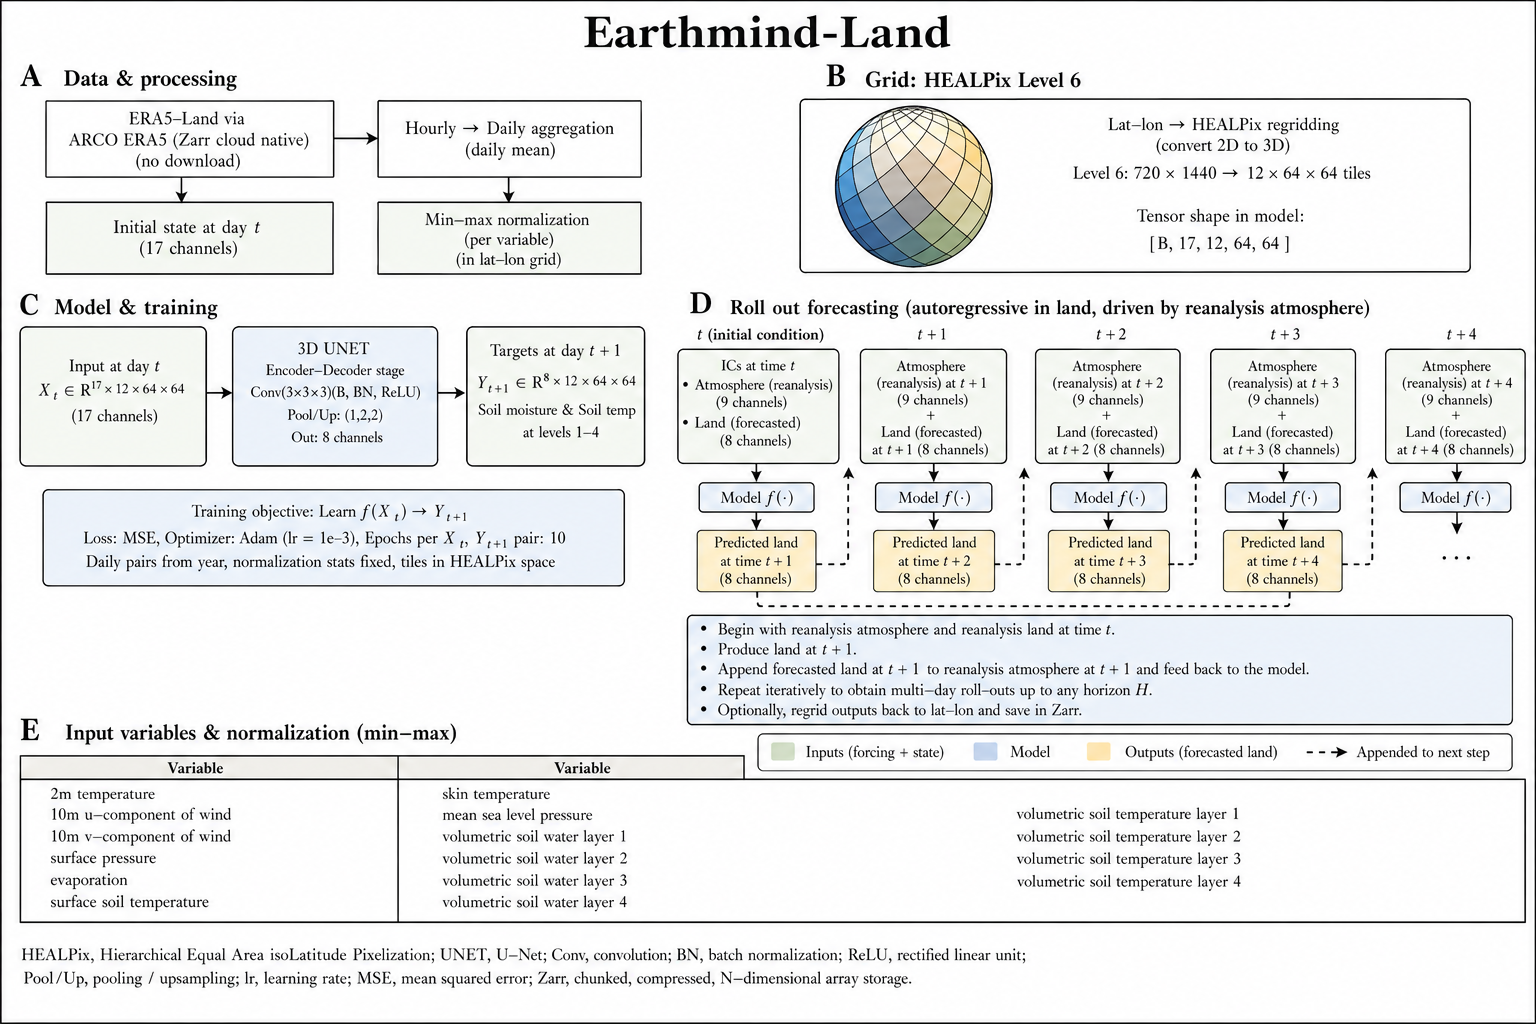
\includegraphics[width=0.8\textwidth]{ai_land_model_schematic_v1.png}
    \caption{Architecture of the Earthmind-Land model.}
    \label{fig:architecture}
\end{figure}

\subsection{Training and Inference}

The model is trained on years 2018--2020 using MSE loss and the Adam optimizer. Inference proceeds autoregressively, where the predicted soil state at each step becomes the input for the next, while atmospheric forcing is prescribed from ERA5 (offline mode).

% =====================================================================
\section{Results}
\label{sec:results}

Short-range forecasts (1--9 days) show high spatial fidelity in capturing global soil moisture and temperature patterns. Extended-range 60-day forecasts across four extreme events (2019 flooding, 2012 drought, 2021 heatwave, 2011 drought) demonstrate the model's S2S-scale skill.

Anomaly correlation coefficients (ACC) for surface soil moisture remain above 0.5 for lead times exceeding 30 days. RMSE growth is consistent with soil moisture memory timescales, with deeper layers exhibiting slower error growth.

% =====================================================================
\section{Discussion and Conclusions}
\label{sec:discussion}

Earthmind-Land is the first standalone modular AI land surface model. It achieves performance comparable to physics-based models in offline validation while being orders of magnitude faster. Its HEALPix-based design ensures compatibility with companion AI atmosphere and ocean models, paving the way for fully coupled AI Earth system forecasting.

\section*{Open Research}

The ERA5 reanalysis data used in this study are available from the ARCO-ERA5 Zarr store on Google Cloud Storage. Code and trained weights are available at \url{https://github.com/manmeet3591/ai_land_model}.

\section*{Acknowledgments}

We thank the Texas Advanced Computing Center (TACC) for computational resources.

\bibliography{references}

\end{document}
